%!TEX root = ../Thesis.tex

\chapter{Anhang - Verwendete Datensätze}
\label{cha:anhang_a}

Nachfolgend sind Aufnahmen der in dieser Arbeit verwendeten Luftaufnahmen zu sehen.

\subsection*{Datensatz Entennest}

\begin{figure}[H]
\centering
    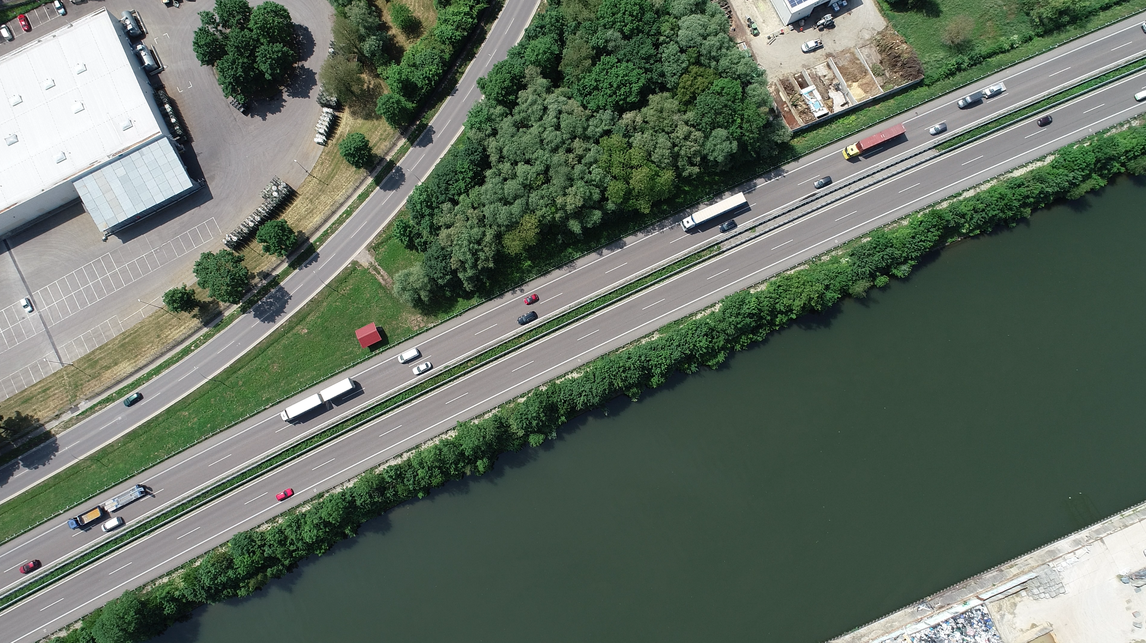
\includegraphics[width=0.6\linewidth]{resources/img/Anhang/Entennest}
\caption{Staßenabschnitt Aufnahme Entennest}
\label{fig:anhang_ds_entennest}
\end{figure}

\subsection*{Datensatz Neckartor}

\begin{figure}[H]
\centering
    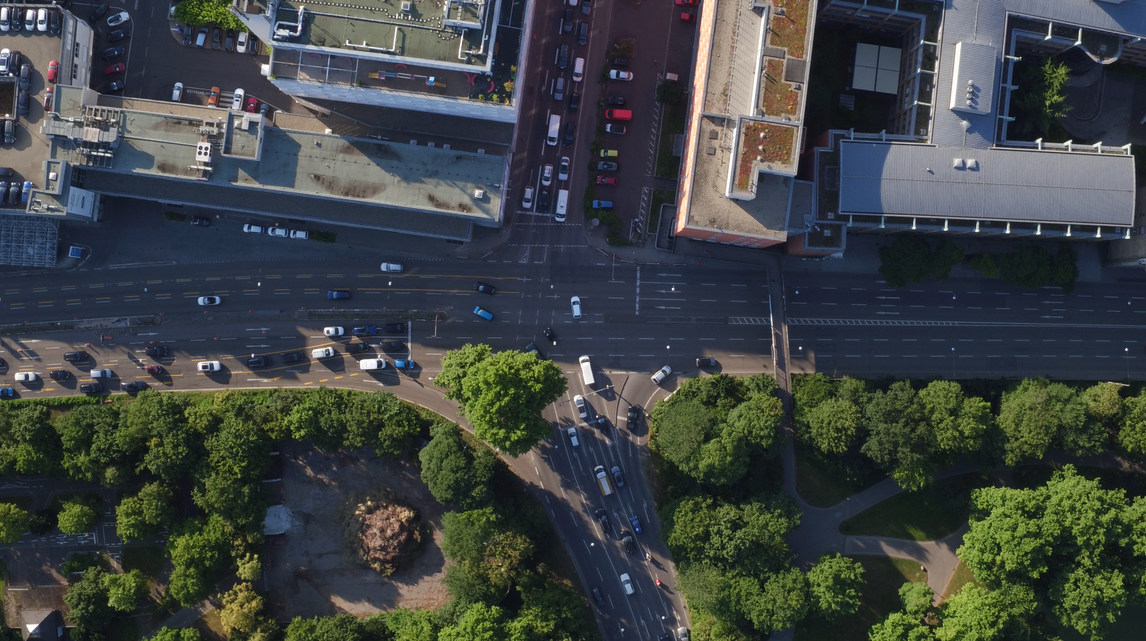
\includegraphics[width=0.6\linewidth]{resources/img/Anhang/Neckartor}
\caption{Staßenabschnitt Aufnahme Neckartor}
\label{fig:anhang_ds_neckartor}
\end{figure}

\subsection*{Datensatz Heilbronner-Straße}

\begin{figure}[H]
\centering
    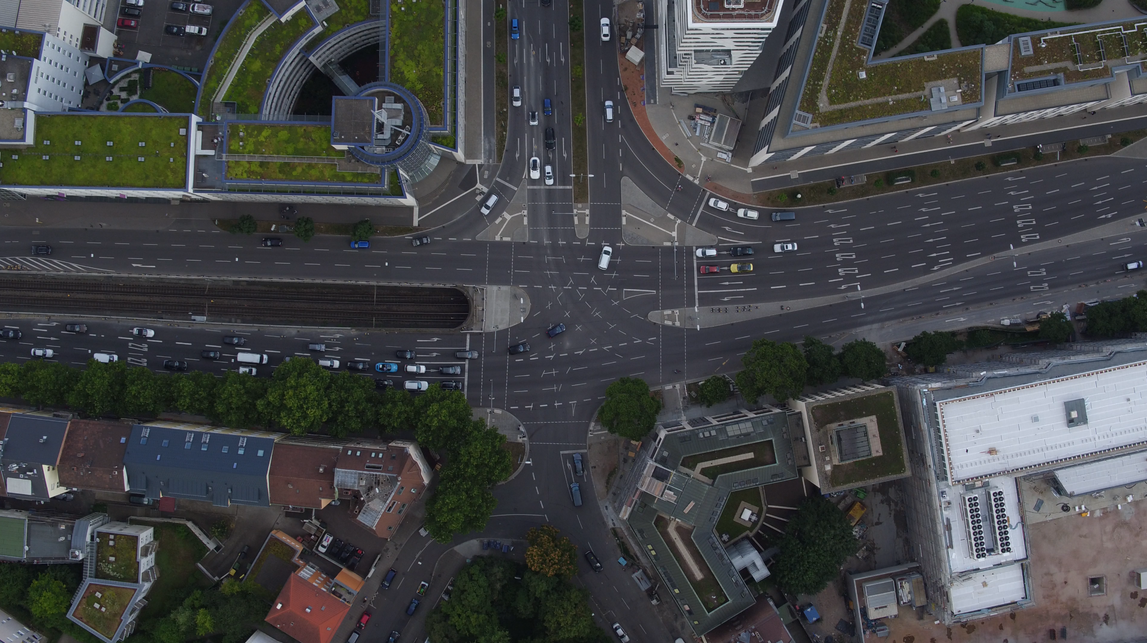
\includegraphics[width=0.6\linewidth]{resources/img/Anhang/Heilbronner}
\caption{Staßenabschnitt Aufnahme Heilbronner-Straße}
\label{fig:anhang_ds_heilbronner}
\end{figure}

\subsection*{Datensatz Düsseldorf}

\begin{figure}[H]
\centering
    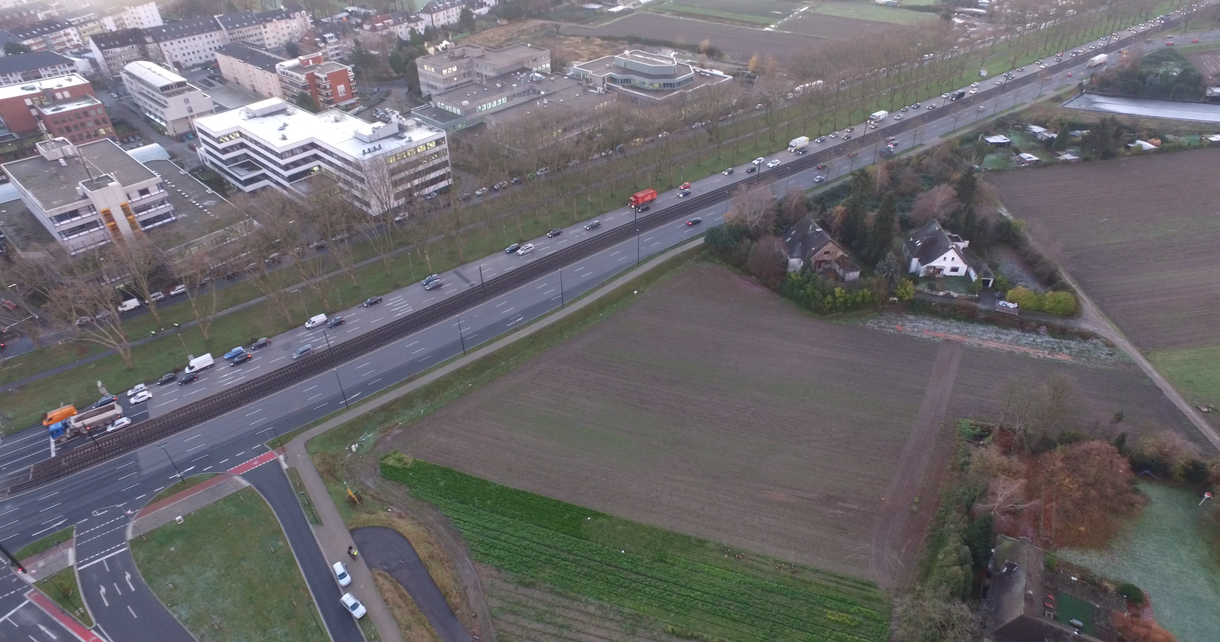
\includegraphics[width=0.6\linewidth]{resources/img/Anhang/Duesseldorf}
\caption{Staßenabschnitt Aufnahme Düsseldorf}
\label{fig:anhang_ds_duesseldorf}
\end{figure}

\subsection*{Datensatz Steinheim}

\begin{figure}[H]
\centering
    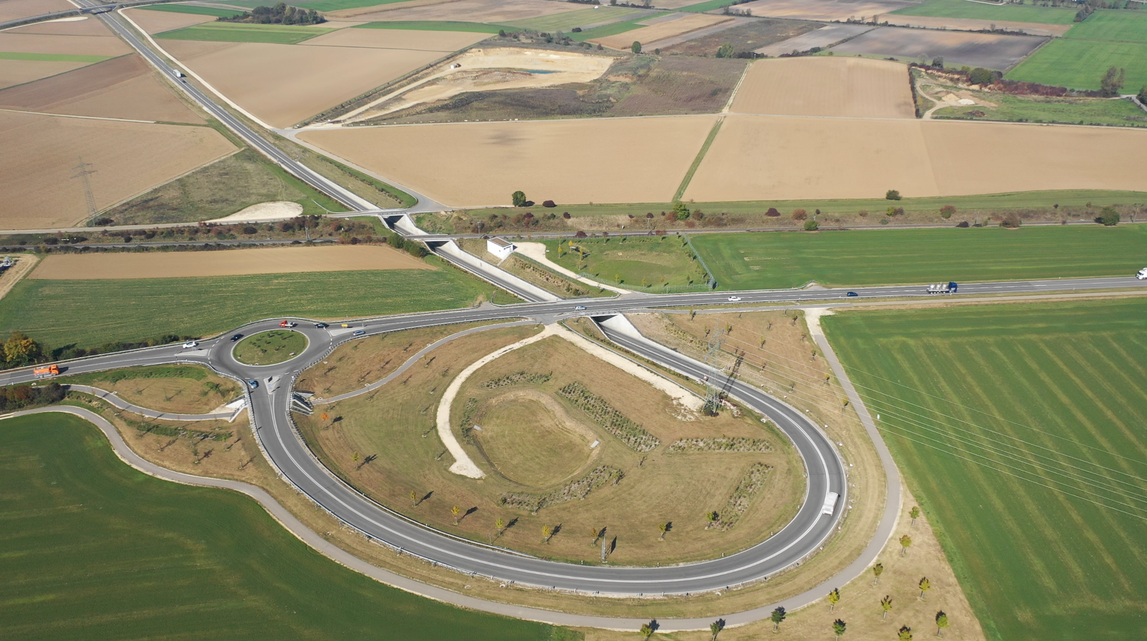
\includegraphics[width=0.6\linewidth]{resources/img/Anhang/Steinheim}
\caption{Staßenabschnitt Aufnahme Steinheim}
\label{fig:anhang_ds_steinheim}
\end{figure}